\documentclass[../../main.tex]{subfiles}

\begin{document}
\subsection{Tree Tensor Networks}
    Now, we want to analyze the properties of these binary tree tensor networks further. It may not bother us how we construct increasingly bigger models that satisfy the bulk marginal property, we know that the model space of binary tree tensor networks is capable of producing a family of networks that satisfy this property.

    Furthermore, we may also constrain every tensor network to be non-negative and normalized. Of course, such networks are always constructable as well. We also allow for negative entries in the tensors. We also don't apply any function $f$ to the tensor output, the network outputs directly correspond to probabilities.

    One question we might ask is whether such a model space restricts the space of possible probability distributions, and if so by how much. As it turns out, in the most general case when allowing very large tensors in the networks, we can model \emph{any} probability distribution:

    \begin{proposition}
        Given any probability distribution $p: \Sigma^{2^k} \mapsto [0,1]$, we can always construct a binary tree tensor network $\mathcal{T}$ over $\Sigma^{2^k}$ s.t. $p \equiv S_{2^k, \mathcal{T}}$ (, where $\mathcal{T}$ has the properties like discussed above and has no constrains on the tensor sizes).
    \end{proposition}
    \vspace{-2.5em}
    \begin{proof}
        For clarity reasons, we only show how to construct $\mathcal{T}$ for $n = 2^k = 4$. The procedure can easily be extended to the general case.

        Our model structure is depicted in figure~\ref{fig:binary_tree_tensor_network_n_equals_four}.

        \begin{figure}[h]
        \centering
        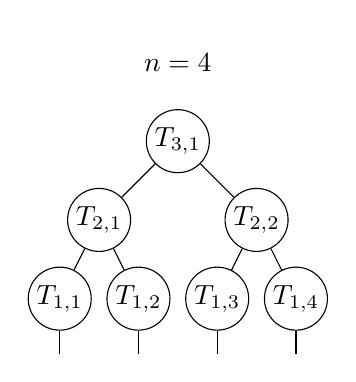
\begin{tikzpicture}[
            every node/.style={circle, draw, minimum size=8mm, inner sep=0pt},
            level distance=10mm,
            sibling distance=10mm,
            edge from parent/.style={draw},
            level 1/.style={sibling distance=20mm},
            level 2/.style={sibling distance=10mm}
        ]

        % Tree with 4 leaves
        \node[draw=none] at (1,0) {$n=4$};
        \node (t31) at (1, -1) {$T_{3,1}$} [grow=down]
        child {node (t21a) {$T_{2,1}$}
            child {node (t11c) {$T_{1,1}$}}
            child {node (t13) {$T_{1,2}$}}}
        child {node (t22) {$T_{2,2}$}
            child {node (t14) {$T_{1,3}$}}
            child {node (t15) {$T_{1,4}$}}};
        \draw (t11c) -- ++(0,-0.7);
        \draw (t13) -- ++(0,-0.7);
        \draw (t14) -- ++(0,-0.7);
        \draw (t15) -- ++(0,-0.7);

        \end{tikzpicture}
        \caption{Model structure of binary tree tensor networks for $n = 2^k = 4$.}
        \label{fig:binary_tree_tensor_network_n_equals_four}
    \end{figure}

    Now, we initialize the leaf matrices as identity matrices $\delta_2 \in \mathbb{R}^{|\Sigma| \times |\Sigma|}$. Thus, when contracting a leaf tensor with a one-hot encoded input vector at position $i$, we get the vector $v_j = \bm{1}[X_i = c_j], c_j \in \Sigma$.

    Now, the tensors in layer two are of the following form:
    \[
    T_{2, j}: |\Sigma| \times |\Sigma| \mapsto \mathbb{R}^{|\Sigma|^2} \quad .
    \]
    The outgoing axis may be index by $(X'_i, X'_{i + 1}) \in \Sigma^2$. The map is then defined by
    \[
        T_{2, j}(X_i, X_{i + 1}) = \bm{1}[(X'_i, X'_{i + 1}) = (X_i, X_{i + 1})] \quad ,
    \]
    i.e. $T_{2, j}$ is a three dimensional tensor with $|\Sigma| \times |\Sigma|$ many vectors of size $|\Sigma|^2$ which are one-hot encoded vectors of 2-tuples of $\Sigma^2$.

    Finally, $T_{3, 1}$ stores the entire probability distribution:
    \[
        T_{3, 1}: |\Sigma|^2 \times |\Sigma|^2 \mapsto [0, 1], ((X'_1, X'_2), (X'_3, X'_4)) \mapsto p(X'_1, X'_2, X'_3, X'_4) \quad .
    \]
    Thus, based on the construction we see that upon contracting the network with an initialization defined by $w \in \Sigma^4$, we get $S_{4, \mathcal{T}}(w) = p(w)$ as desired.

    Note that this construction can easily be extended to arbitrary $n = 2^k$.
    \end{proof}

    As one might expect, we see that our general construction needs $\Omega(|\Sigma|^n)$ many parameters because the root tensor stores all the $|\Sigma|^n$ many probabilities for $w \in \Sigma^n$. Of course, there cannot be a general model capable of any probability distribution with $o(|\Sigma|^n)$ many parameters.

\end{document}